\chapter{Metode Penelitian}

\section{Alat Tugas Akhir}

Penelitian ini berbasis model yang disusun dan disimulasikan di perangkat lunak MATLAB versi 2024a, khususnya menggunakan skrip pemrograman dan Simscape pada Simulink. Simscape mencakup pustaka \textit{Specialized Power System} untuk pemodelan sistem tenaga listrik dan elektronika daya berdasarkan bentuk nyata.




\section{Pemodelan Sistem}



\subsection{Model Sistem SPV}

Sistem SPV terdiri dari \textit{solar array} yang tersusun seri dan paralel dari banyak sel surya dan DC-DC \textit{Boost Converter} yang dikendalikan oleh MPPT untuk menentukan titik daya maksimum. Selain itu terdapat kapasitor DC link, serta inverter 3 fasa. \textit{Solar array} menghhasilkan tegangan DC sampai ke DC link. DC link akan dijaga tegangannya oleh BESS, yang terdiri dari baterai dan \textit{Bidirectional} DC-DC \textit{Buck-Boost Converter}. Lalu, inverter akan mengubah tegangan DC menjadi AC yang sinkron dengan jaringan.

\begin{figure}[ht]
	\centering
	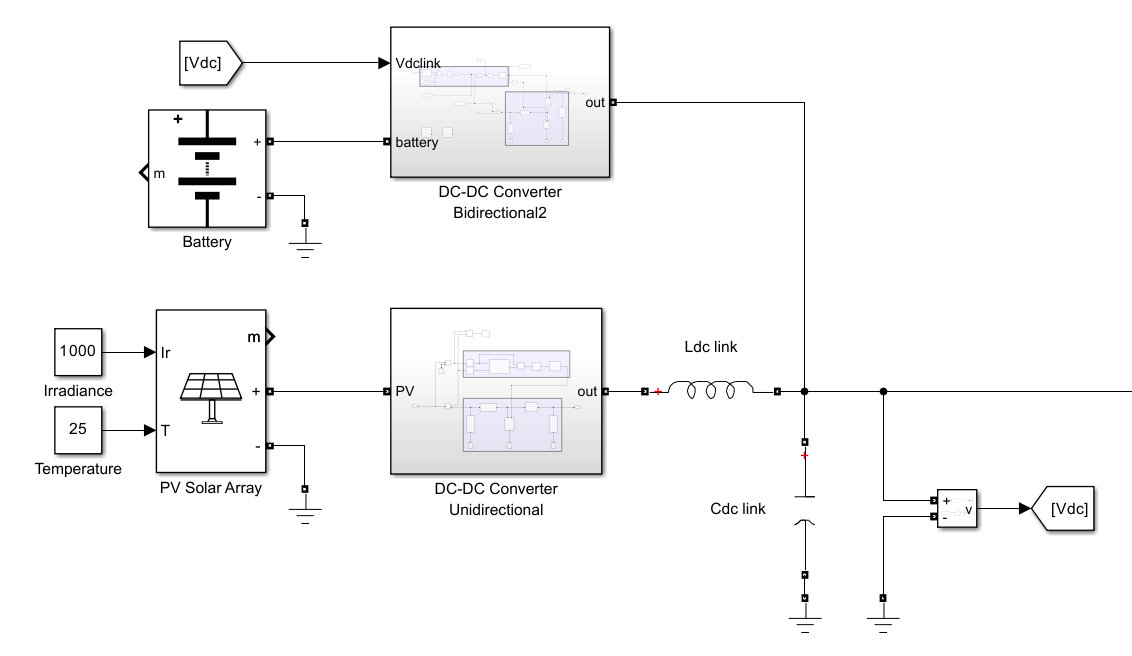
\includegraphics[width=12cm]{contents/chapter-3/model_spv.png}
	\caption{Diagram Blok Simulink Sistem SPV}
	\label{Fig:spv}
\end{figure}

Dalam penelitian ini, iradiasi matahari dan temperatur dianggap konstan sebesar $\mathit{1 \ kW/m^2}$ dan $\mathit{25 ^\circ C}$ karena fokus penelitian berada pada analisis stabilitas transien. Maka dari itu, daya keluaran dari sistem SPV ditentukan pada titik operasi $\mathit{1,5 \ MW}$ sebagai referensi daya inverter dari \textit{rating} daya maksimal $\mathit{2 \ MW}$ selama simulasi berlangsung. Selain itu, konverter DC-DC dan Inverter disimulasikan dengan model \textit{detailed switching}.



\subsubsection{MPPT dan DC-DC \textit{Boost Converter}}

\begin{figure}[ht]
	\centering
	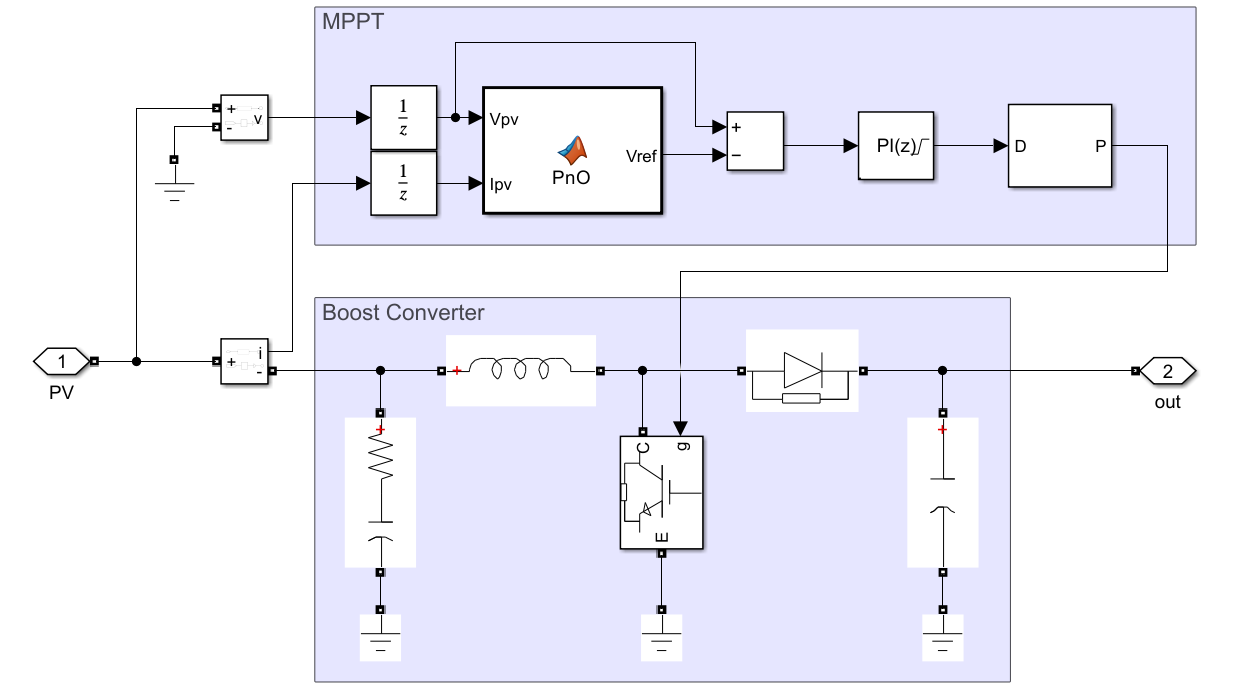
\includegraphics[width=12cm]{contents/chapter-3/mppt.png}
	\caption{Diagram Blok Simulink MPPT dan DC-DC \textit{Boost Converter}}
	\label{Fig:mppt}
\end{figure}

MPPT menggunakan algoritma Perturb and Observe (P\&O) akan terus melakukan iterasi untuk mencari titik daya maksimum yang dapat dihasilkan oleh \textit{solar array} berdasarkan kombinasi nilai tegangan dan arus dari \textit{solar array}. P\&O memberikan referensi tegangan untuk mengontrol \textit{switching} DC-DC \textit{Boost Converter}.

\begin{equation}
	\mathit{e_{V,PV}} = V_{PV} - P\&O(V_{PV}, I_{PV})
\end{equation}
\begin{equation}
	\mathit{u_{ref,PV}} = K_{P,PV}e_{V,PV} + K_{I,PV}\int e_{V,PV}dt
\end{equation}

\begin{table}[ht]
	\caption{Tabel Parameter MPPT dan DC-DC \textit{Boost Converter}}
	\vspace{0.5em}
	\centering
	\begin{tabular}{|c|c|c|}
		\hline
		Parameter & Nilai & Satuan \\
		\hline
		$\mathit{P_{PV}}$ & 2 & MW \\
		$\mathit{V_{PV}}$ & 0,9 - 1 & kV \\
		$\mathit{V_{DC,link}}$ & 1,5 & kV \\
		$\mathit{L}$ & 16,13 & mH \\
		$\mathit{C}$ & 94,8 & mF \\
		\hline
	\end{tabular}
	\label{Tab: tabel mppt}
\end{table}



\subsubsection{BESS}

\begin{figure}[ht]
	\centering
	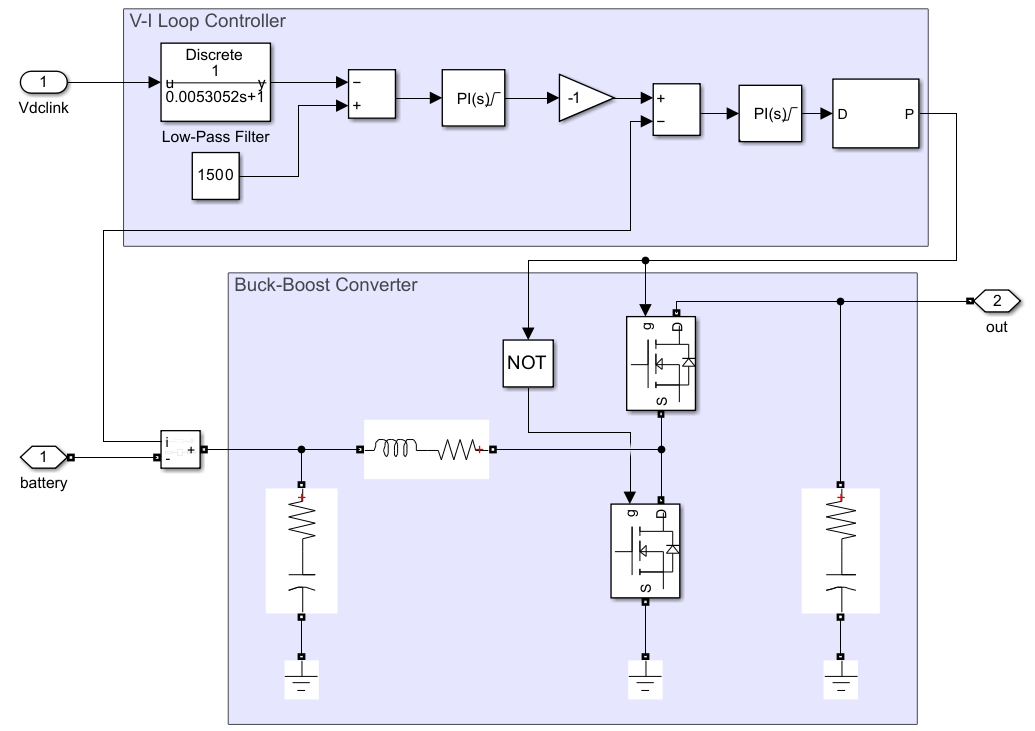
\includegraphics[width=12cm]{contents/chapter-3/bess.png}
	\caption{Diagram Blok Simulink BESS }
	\label{Fig:bess}
\end{figure}

BESS berperan sebagai sumber daya tambahan untuk menjaga keseimbangan daya pada DC \textit{link}. Ketidakseimbangan daya yang disebabkan karena adanya perbedaan antara daya keluaran \textit{solar array} dan referensi daya inverter dapat menyebabkan tegangan DC \textit{link} berubah, yang dapat mempengaruhi kinerja dan kestabilan inverter. BESS akan menyuplai atau menyerap daya aktif dengan cepat selama terdapat deviasi tegangan DC \textit{link} dari nilai nominalnya. 

Baterai pada BESS dimodelkan dengan tipe \textit{lead-acid}.Konverter memungkinkan aliran daya 2 arah, sehingga baterai dapat melakukan \textit{charging} ataupun \textit{discharging} sesuai kebutuhan berdasarkan status deviasi tegangan DC \textit{link}.

\begin{equation}
	\mathit{e_{V,dclink}} = V_{DC,link} - 1500
\end{equation}
\begin{equation}
	\mathit{i_{ref,BESS}} = K_{P,BESS}e_{V,dclink} + K_{I,BESS}\int e_{V,dclink}dt
\end{equation}
\begin{equation}
	\mathit{e_{i,bat}} = i_{ref,BESS} - i_{bat}
\end{equation}
\begin{equation}
	\mathit{i_{ref,bat}} = K_{P,bat}e_{i,bat} + K_{I,bat}\int e_{i,bat}dt
\end{equation}

\begin{table}[ht]
	\caption{Tabel Parameter BESS}
	\vspace{0.5em}
	\centering
	\begin{tabular}{|c|c|c|}
		\hline
		Parameter & Nilai & Satuan \\
		\hline
		$\mathit{Q_{bat}}$ & 2 & kAh \\
		$\mathit{V_{bat}}$ & 750 & V \\
		$\mathit{R_{bat,int}}$ & 20 & m$\Omega$ \\
		$\mathit{L}$ & 1,9 & mH \\
		$\mathit{C_{buck}}$ & 1,3 & mF \\
		$\mathit{C_{boost}}$ & 66,7 & mF \\
		\hline
	\end{tabular}
	\label{Tab: tabel bess}
\end{table}



\subsection{Model Inverter}

\begin{figure}[ht]
	\centering
	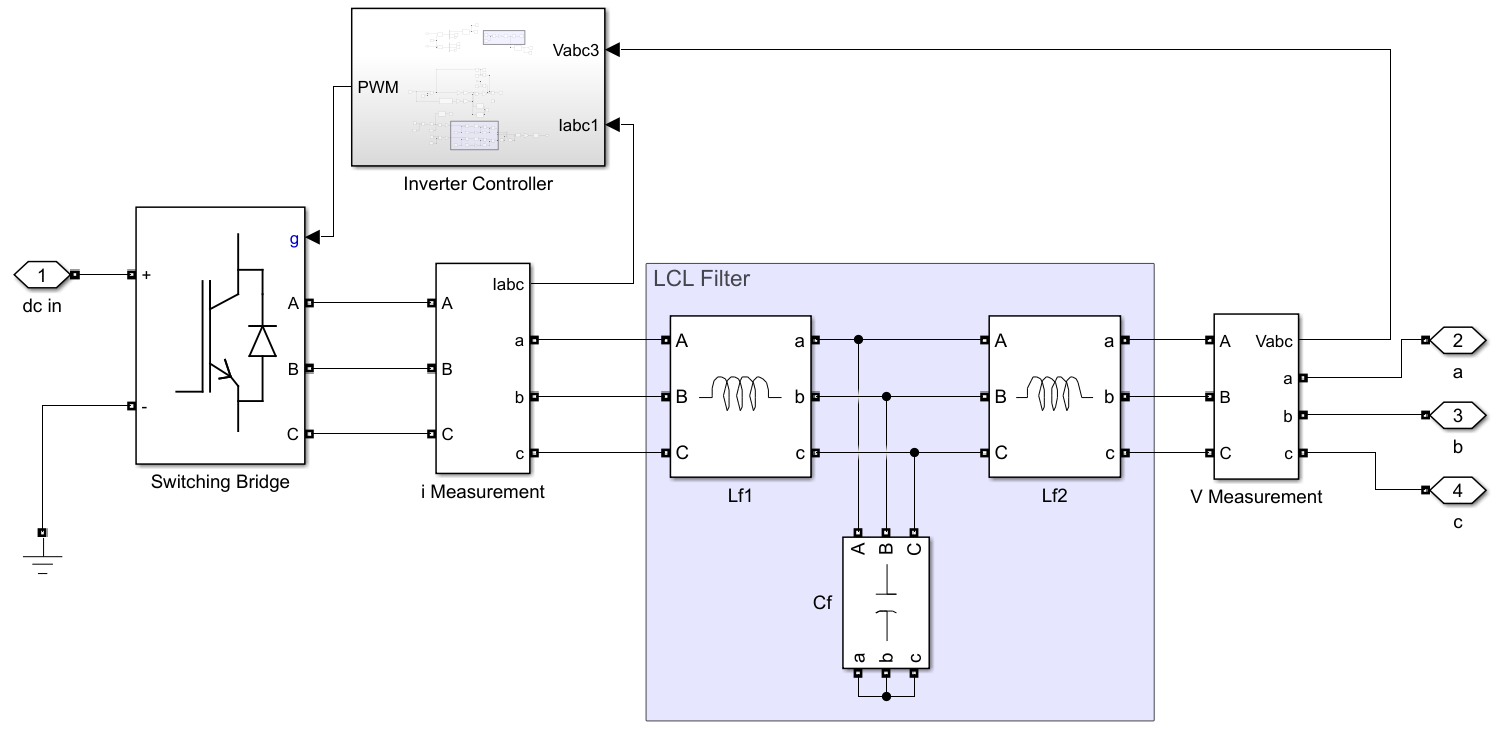
\includegraphics[width=12cm]{contents/chapter-3/inverter.png}
	\caption{Diagram Blok Simulink Inverter}
	\label{Fig:inverter}
\end{figure}

Inverter 3 fasa dimodelkan sebagai \textit{grid-following (GFL)} dengan topologi \textit{full-bridge}. Inverter bertugas untuk mengubah tegangan $\mathit{1,5 \ kV_{DC}}$ menjadi $\mathit{800 \ V_{AC,peak-peak}}$ yang kemudian dinaikkan tegangannya menjadi $\mathit{345 \ kV_{AC,peak-peak}}$ agar sesuai dengan level tegangan jaringan.


\subsubsection{Sinkronisasi}

\begin{figure}[ht]
	\centering
	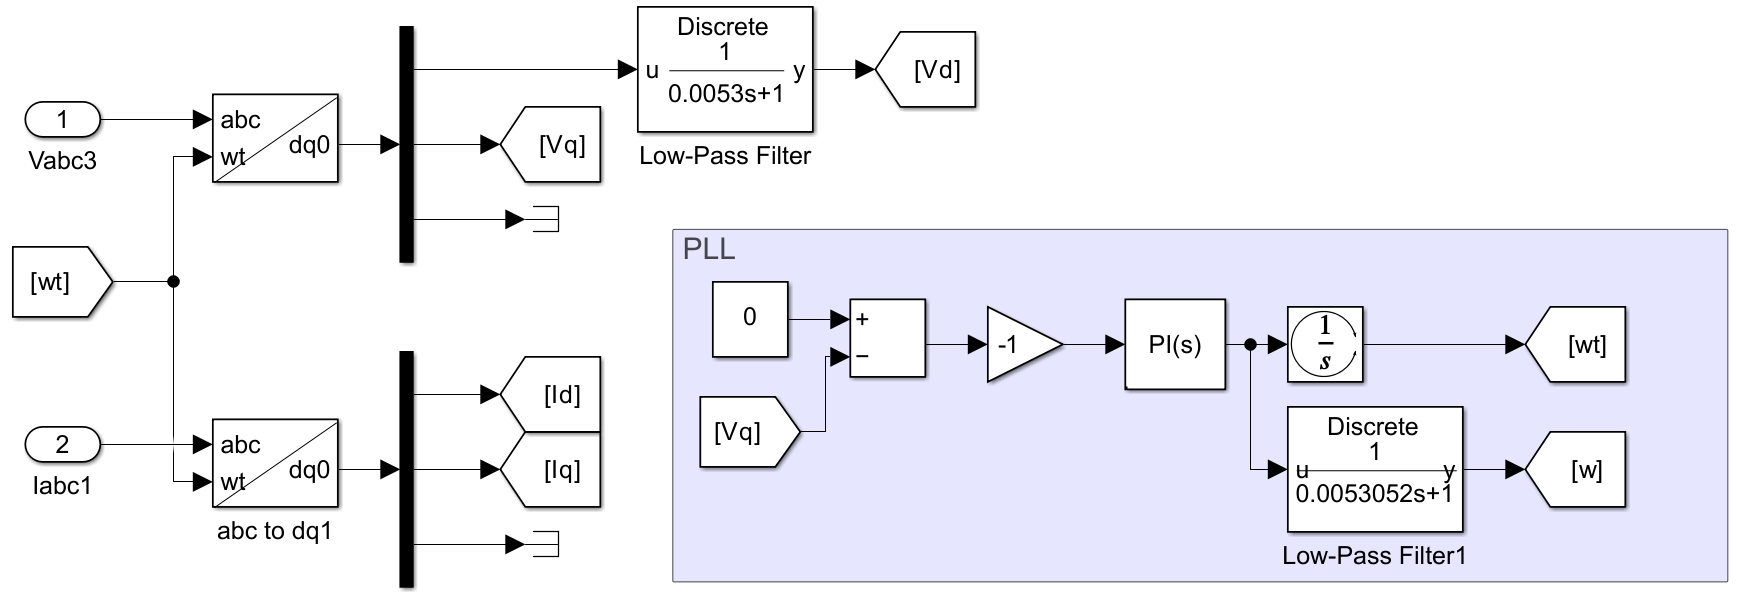
\includegraphics[width=12cm]{contents/chapter-3/pll.png}
	\caption{Diagram Blok Simulink PLL }
	\label{Fig:pll}
\end{figure}

Inverter disinkronkan dengan jaringan menggunakan PLL. Kemudian, untuk menyederhanakan sistem kontrol, sinyal AC (sumbu abc) yang didapat dari sensor di jaringan, akan ditransformasikan menggunakan transformasi Park untuk mengubah sinyal AC menjadi sinyal DC (sumbu dq) pada tegangan maupun arus, sehingga akan mendapatkan 4 variabel $\mathit{V_d}$, $\mathit{V_q}$, $\mathit{i_d}$, dan $\mathit{i_q}$. $\mathit{V_d}$ merepresentasikan tegangan puncaknya, sedangkan $\mathit{V_q}$ akan dimanfaatkan oleh PLL dalam sinkronisasi untuk menyamakan fasa antara inverter dengan jaringan. PLL juga nantinya akan digunakan untuk kontrol virtual inertia sebagai sensor frekuensi. 

\begin{equation}
	\mathit{\omega_{PLL}} = K_{P,PLL}V_q + K_{I,PLL}\int V_q dt	
\end{equation}
\begin{equation}
	\mathit{\theta_{PLL}} = \int \omega_{PLL} dt = \omega_{PLL}t
\end{equation}


\subsubsection{Kontrol Inverter}

\begin{figure}[ht]
	\centering
	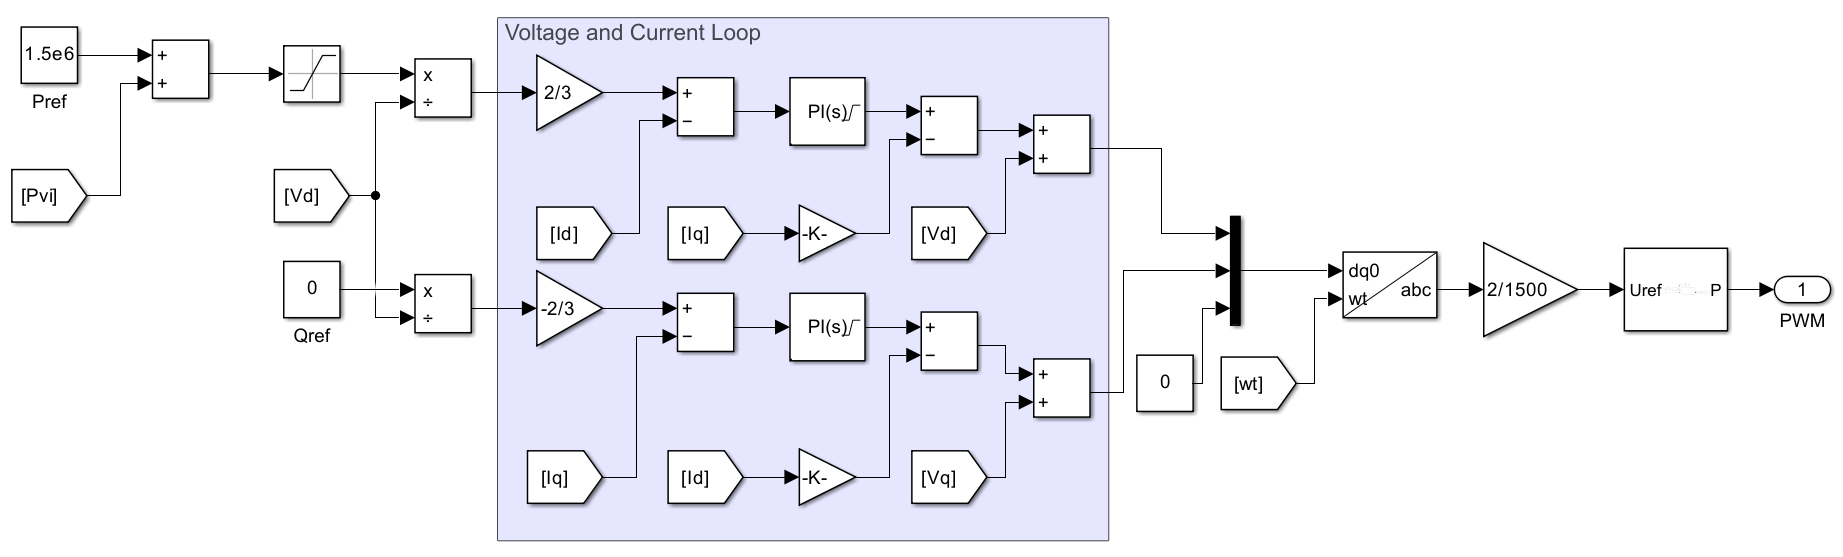
\includegraphics[width=12cm]{contents/chapter-3/kontrol_inverter.png}
	\caption{Diagram Blok Simulink Kontrol Inverter }
	\label{Fig:kontrol inverter}
\end{figure}

Menggunakan persamaan dari [] pada persamaan \ref{Eq: idiq kontrol inverter} dan \ref{Eq: VdVq kontrol inverter}, tegangan dan arus dapat dikontrol agar daya keluaran akan menyesuaikan dengan referensi daya aktif dan reaktif yang diberikan. $\mathit{i_d}$ berperan untuk mengontrol daya aktif, sedangkan $\mathit{i_q}$ mengontrol daya reaktif. $\mathit{P_{VI}}$ pada gambar \ref{Fig:kontrol inverter} adalah daya akibat virtual inertia yang akan dijelaskan pada bagian \ref{sec:virtual inertia}.


\begin{equation}
\begin{aligned}
    i_{d,ref} &= \frac{2}{3} \frac{P_{ref}+P_{VI}}{V_d} \\
    i_{q,ref} &= -\frac{2}{3} \frac{Q_{ref}}{V_d}
\end{aligned}
\label{Eq: idiq kontrol inverter}
\end{equation}

\begin{equation}
\begin{aligned}
    V_{d,ref} &= PI(i_{d,ref}-i_d) - 2i_q\omega_nL_{inv} + V_d \\
    V_{q,ref} &= PI(i_{q,ref}-i_q) - 2i_d\omega_nL_{inv} + V_q
\end{aligned}
\label{Eq: VdVq kontrol inverter}
\end{equation}


\subsubsection{Filter LCL}

Pada Gambar \ref{Fig:inverter}, terdapat filter LCL yang terdiri dari induktor dan kapasitor. Filter LCL yang merupakan bagian dari LPF digunakan untuk meredam komponen harmonik dari \textit{switching} sehingga sinyal keluaran berupa sinusiodal yang lebih bersih dari distorsi.

\begin{table}[ht]
	\caption{Tabel Parameter Filter LCL}
	\vspace{0.5em}
	\centering
	\begin{tabular}{|c|c|c|}
		\hline
		Parameter & Nilai & Satuan \\
		\hline
		$\mathit{\omega_n}$ & 314,16 & rad/s \\
		$\mathit{L}$ & 14,13 & mH \\
		$\mathit{C}$ & 22,4 & $\mu$F \\
		\hline
	\end{tabular}
	\label{Tab: tabel filter lcl}
\end{table}



\subsection{Model Kontroler \textit{Virtual Inertia}}
\label{sec:virtual inertia}

\begin{figure}[ht]
	\centering
	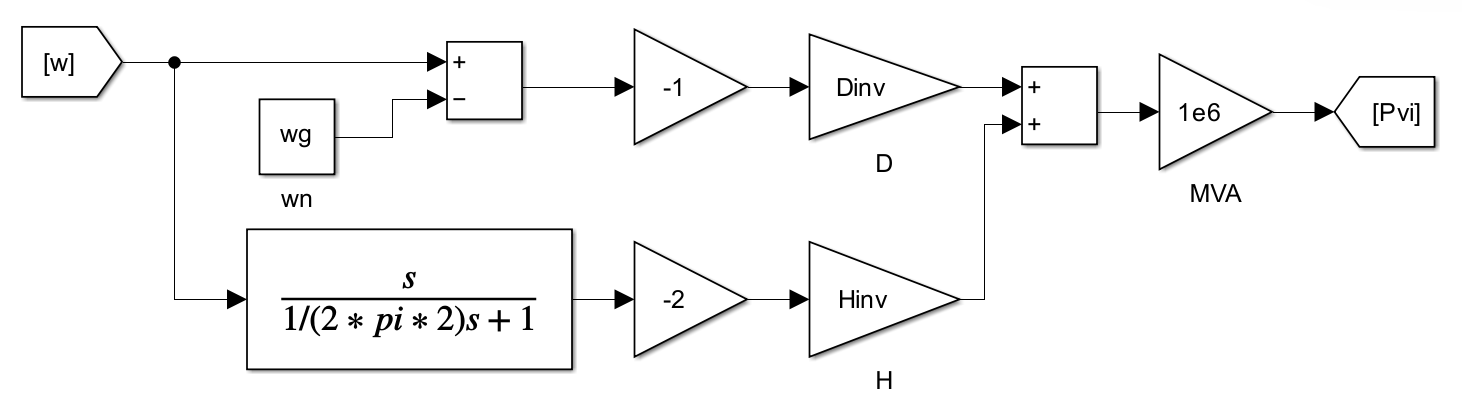
\includegraphics[width=12cm]{contents/chapter-3/vi.png}
	\caption{Diagram Blok Simulink Kontrol Virtual Inertia }
	\label{Fig:virtual inertia}
\end{figure}

\textit{Virtual Inertia} membuat inverter berperilaku seperti generator sinkron yang secara alami mempunyai redaman dan inersia. \textit{Virtual Inertia} dapat merespon perubahan frekuensi pada grid melalui PLL dalam bentuk perubahan daya aktif yang cepat. Redaman dan inersia total pada jaringan akan meningkat sebagai hasil dari kontribusi \textit{Virtual Inertia} pada inverter.

Berdasarkan persamaan ayunan persamaan \ref{Eq: Pswing}, nilai koefisien redaman ($\mathit{D}$) dan konstanta inersia ($\mathit{H}$) juga dapat diimplementasikan ke inverter dalam bentuk penguatan terhadap deviasi dan perubahan frekuensi. Maka dari itu, bisa didapatkan persamaan untuk menghitung daya akibat \textit{virtual inertia} seperti pada persamaan \ref{Eq: PVI}.

\begin{equation}
	2H\frac{d\omega}{dt} = P_m-P_e -D(\omega - \omega_n)
\label{Eq: Pswing}
\end{equation}
Definisikan $\mathit{\Delta P = P_m-P_e}$, lalu pindah ruas
\begin{equation}
	\Delta P = 2H\frac{d\omega}{dt} + D(\omega - \omega_n)
\end{equation}
Pada virtual inertia, inverter memberikan daya kompensasi yang arahnya melawan perubahan frekuensi, maka
\begin{equation}
	P_{VI} = -\Delta P
\end{equation}
\begin{equation}
	P_{VI} = -2H_{virt}\frac{d\omega}{dt} -D_{virt}(\omega - \omega_n)
\label{Eq: PVI}
\end{equation}
Sehingga, referensi daya aktif pada inverter akan menjadi
\begin{equation}
	P_{ref} = P_{ref,0} + P_{VI}
\end{equation}
\begin{equation}
	P_{ref} = P_{ref,0} -2H_{virt}\frac{d\omega}{dt} -D_{virt}(\omega - \omega_n)
\end{equation}

Referensi daya aktif pada kontroler inverter dibatasi oleh \textit{rating} daya inverter. Pembacaan frekuensi dari PLL beserta turunannya dilewatkan LPF untuk menghilangkan \textit{noise} untuk mengurangi risiko kesalahan pada kontroler.

Pada pemodelan \textit{virtual inertia} ini, nilai parameter redaman virtual ($\mathit{D_{virt}}$) dan konstanta inersia virtual ($\mathit{H_{virt}}$) ditentukan nilainya adalah 1 p.u. dan 2 s. Sedangkan nilai konstanta waktu pada LPF adalah 0,08 s. Konstanta waktu pada LPF juga harus diperhatikan untuk menghindari respon yang terlalu lambat.



\subsection{Model Jaringan}

Jaringan terdiri dari 3 bus, masing-masing bus terdapat generator sinkron dan beban. Bus 3 dianggap sebagai \textit{slack bus}. Bus dihubungkan dengan saluran ke kedua bus lainnya.


\subsubsection{Generator Sinkron}

Generator sinkron pada penelitian ini akan menggunakan model orde 2 yang dioperasikan di titik operasi tertentu. Ketiga generator mempunyai basis daya yang sama, yaitu $\mathit{1 \ MVA}$. 3 Generator akan dipasang di 3 titik bus yang berbeda.

\begin{table}[ht]
	\caption{Tabel Parameter Generator Sinkron}
	\vspace{0.5em}
	\centering
	\begin{tabular}{|c|c|c|c|c|}
		\hline
		$\mathit{G_i}$ & $\mathit{P_m \ (pu)}$ & $\mathit{D \ (pu)}$ & $\mathit{H \ (pu)}$ & $\mathit{x'_d \ (pu)}$ \\ 
		\hline
		1 & 2,49 & 10 & 7 & $\mathit{j}$0,088 \\
		2 & 4,21 & 10 & 8 & $\mathit{j}$0,050 \\
		3 & 8,20 & 10 & 12 & $\mathit{j}$0,015 \\
		\hline
	\end{tabular}
	\label{Tab: tabel gen}
\end{table}


\subsubsection{Saluran}

Pada model ini, hanya ada kontribusi reaktansi pada saluran. Sehingga dianggap \textit{lossless}, yang berarti tidak ada resistansi di sepanjang saluran.

\begin{table}[ht]
	\caption{Tabel Parameter Saluran}
	\vspace{0.5em}
	\centering
	\begin{tabular}{|c|c|c|}
		\hline
		From bus & To bus & $\mathit{X \ (pu)}$ \\
		\hline
		1 & 2 & $\mathit{j}$0,4600 \\
		1 & 3 & $\mathit{j}$0,2600 \\
		2 & 3 & $\mathit{j}$0,0806 \\
		\hline
	\end{tabular}
	\label{Tab: tabel saluran}
\end{table}


\subsubsection{Beban}

Beban diasumsikan sebagai beban konstan PQ dengan komponen resistif dan induktif, yang berarti beban akan menyerap daya aktif dan reaktif senilai titik operasi yang sudah ditentukan.

\begin{table}[ht]
	\caption{Tabel Parameter Beban}
	\vspace{0.5em}
	\centering
	\begin{tabular}{|c|c|c|}
		\hline
		$\mathit{S_{i,load}}$ & $\mathit{P \ (pu)}$ & $\mathit{Q \ (pu)}$ \\
		\hline
		1 & 1,5 & $\mathit{j}$0,4600 \\
		2 & 1,0 & $\mathit{j}$0,2600 \\
		3 & 12,4 & $\mathit{j}$0,0806 \\
		\hline
	\end{tabular}
	\label{Tab: tabel beban}
\end{table}




\section{Validasi model}



\subsection{Konfigurasi sistem dan SLD}

\begin{figure}[ht]
	\centering
	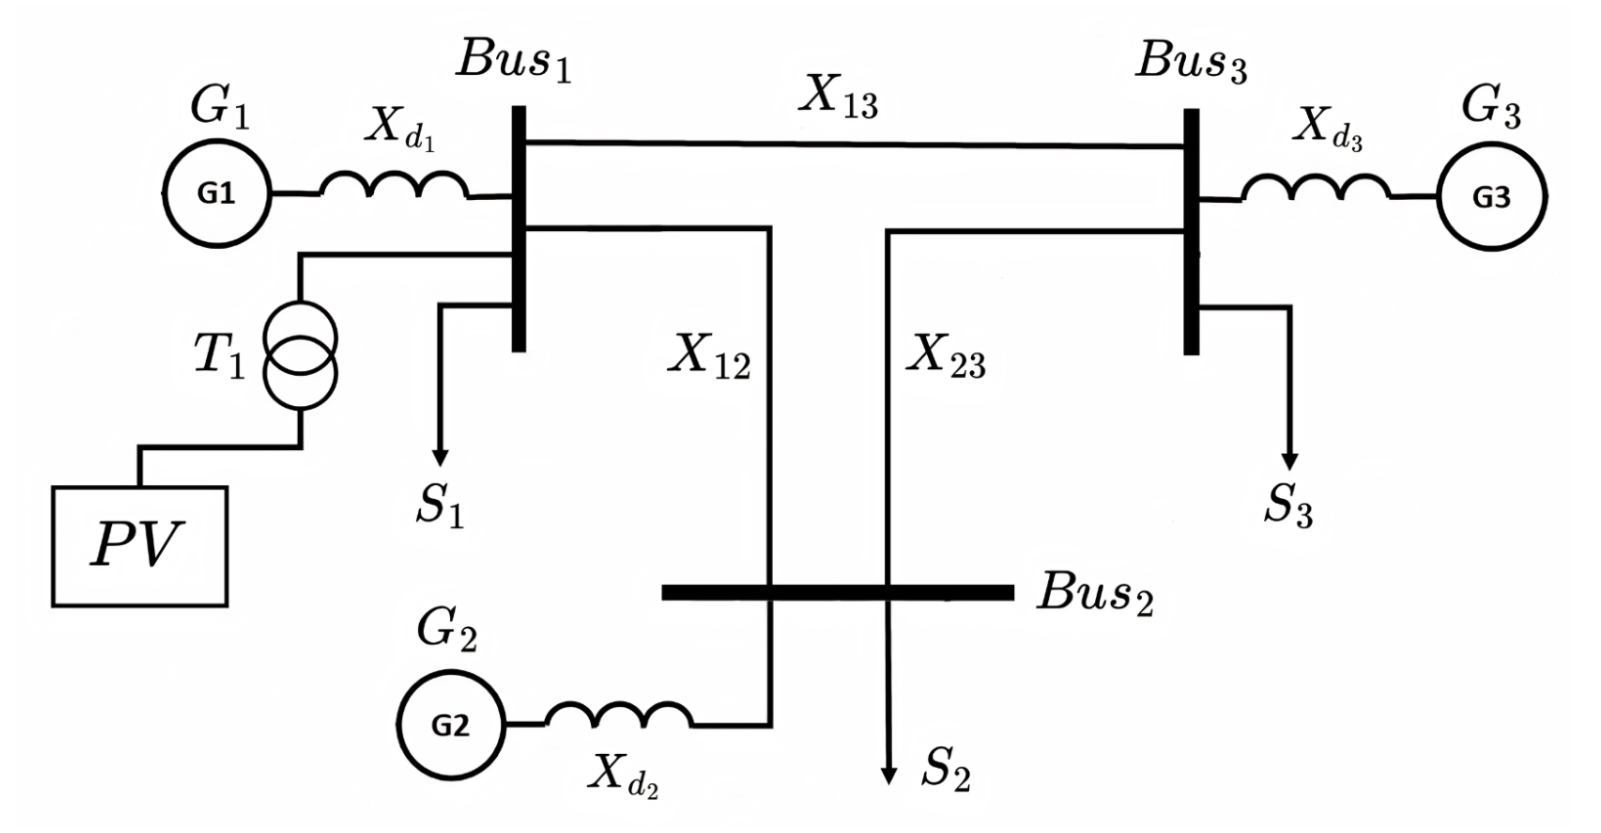
\includegraphics[width=12cm]{contents/chapter-3/sld.png}
	\caption{SLD Jaringan}
	\label{Fig:sld}
\end{figure}

Model pada gambar \ref{Fig:sld} akan digunakan sebagai \textit{baseline} penelitian. Model tersebut adalah hasil modifikasi dari [] yang merupakan studi kasus IEEE 3 bus, dengan modifikasi nilai konstanta redaman dan inersia alami pada generator untuk menonjolkan kontribusi \textit{virtual inertia} pada inverter. Model ini telah digunakan di beberapa penelitian sebelumnya untuk menganalisis stabilitas transien, contohnya []. Model yang sederhana tetapi cukup lengkap, serta bisa menunjukkan fenomena interaksi \textit{multi-machine}.



\subsection{Hasil Aliran Daya}

\subsubsection{\textit{Baseline}}

\begin{figure}[ht]
	\centering
	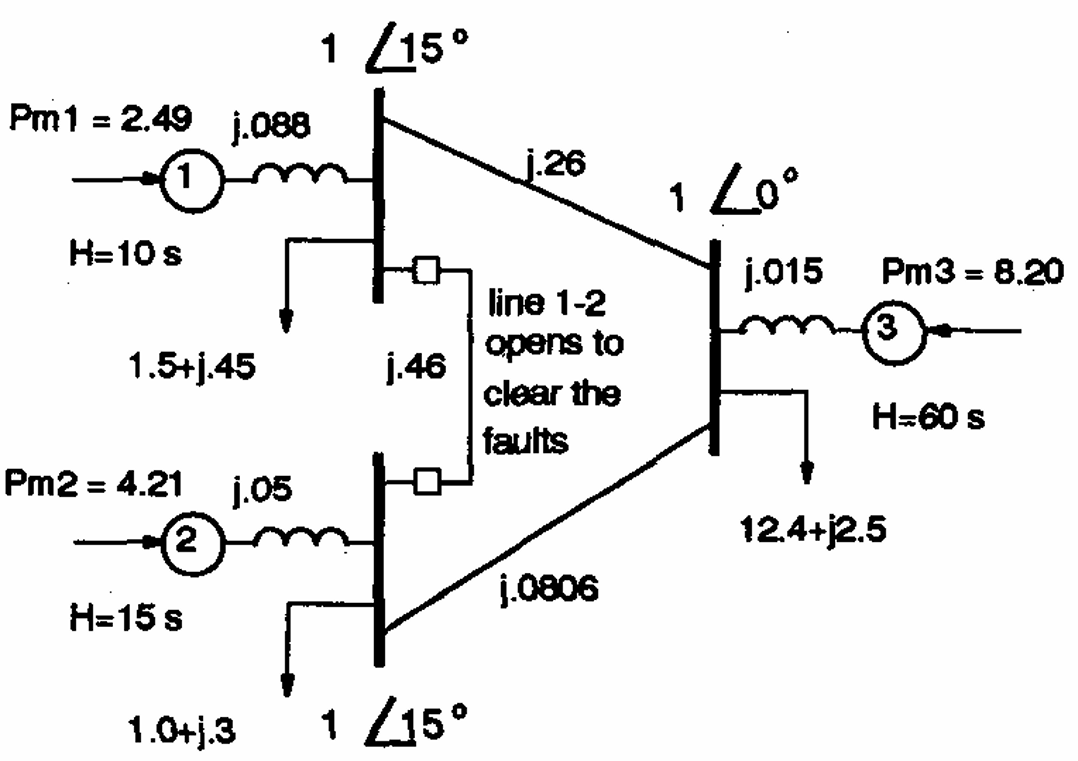
\includegraphics[width=12cm]{contents/chapter-3/sld_ref.png}
	\caption{SLD Jaringan dari []}
	\label{Fig:sld ref}
\end{figure}

\begin{table}[ht]
	\caption{Tabel Hasil Aliran Daya pada \textit{Baseline}}
	\vspace{0.5em}
	\centering
	\begin{tabular}{|c|c|c|c|c|c|c|}
		\hline
		 & $\mathit{P \ (pu)}$ & $\mathit{Q \ (pu)}$ & $\mathit{V_{mag} \ (pu)}$ & $\mathit{V_{ang} \ (^{\circ})}$ & $\mathit{E' \ (pu)}$ & $\delta_{0,rotor} (^{\circ}))$ \\
		\hline
		$\mathit{G_1}$ & 2,49 & 0,580 & 1 & 14,9415 & 1,0736 & 26,71770 \\
		$\mathit{S_{1,load}}$ & 1,50 & 0,450 & 1 & 14,9415 & - & - \\
		$\mathit{G_2}$ & 4,21 & 0,722 & 1 & 14,9860 & 1,0573 & 26,47020 \\
		$\mathit{S_{2,load}}$ & 1,00 & 0,300 & 1 & 14,9860 & - & - \\
		$\mathit{G_3}$ & 8,20 & 3,052 & 1 & 0 & 1,0530 & 6,70815 \\
		$\mathit{S_{3,load}}$ & 12,40 & 2,500 & 1 & 0 & - & - \\
		\hline
	\end{tabular}
	\label{Tab: tabel loadflow baseline}
\end{table}

Model \textit{baseline} yang telah disusun kemudian dianalisis aliran daya, lalu dibandingkan dengan hasil aliran daya dari []. Hal ini dilakukan untuk memastikan bahwa model yang disusun sudah benar dan sesuai dengan kondisi operasi yang diinginkan. Dapat dilihat pada Gambar \ref{Fig:sld ref} dan Tabel \ref{Tab: tabel loadflow baseline} bahwa hasil aliran daya dari model yang disusun sesuai dengan referensi, sehingga model sudah valid untuk digunakan pada analisis selanjutnya.

\subsubsection{\textit{Baseline} dengan SPV}

\begin{table}[ht]
	\caption{Tabel Hasil Aliran Daya pada \textit{Baseline dengan SPV}}
	\vspace{0.5em}
	\centering
	% \small
	\begin{tabular}{|c|c|c|c|c|c|c|}
		\hline
		 & $\mathit{P \ (pu)}$ & $\mathit{Q \ (pu)}$ & $\mathit{V_{mag} \ (pu)}$ & $\mathit{V_{ang} \ (^{\circ})}$ & $\mathit{E' \ (pu)}$ & $\delta_{0,rotor} (^{\circ}))$ \\
		\hline
		$\mathit{G_1}$ & 0,998 & 0,5794 & 1 & 14,9415 & 1,0547 & 19,71820 \\
		$\mathit{S_{1,load}}$ & 1,500 & 0,450 & 1 & 14,9415 & - & - \\
		$\mathit{SPV_{inv}}$ & 1,492 & 6,069 $\cdot 10^{-4}$ & 1 & 14,9415 & - & - \\
		$\mathit{G_2}$ & 4,210 & 0,722 & 1 & 14,9860 & 1,0573 & 26,47020 \\
		$\mathit{S_{2,load}}$ & 1,000 & 0,300 & 1 & 14,9860 & - & - \\
		$\mathit{G_3}$ & 8,200 & 3,052 & 1 & 0 & 1,0530 & 6,70815 \\
		$\mathit{S_{3,load}}$ & 12,400 & 2,500 & 1 & 0 & - & - \\
		\hline
	\end{tabular}
	\label{Tab: tabel loadflow SPV}
\end{table}

Jaringan \textit{baseline} kemudian akan diberikan injeksi sistem SPV. Hal tersebut akan menghasilkan titik operasi baru. Untuk analisis aliran daya pada kasus ini, SPV dimodelkan sebagai beban negatif PQ. Hasil aliran daya yang baru dapat dilihat pada tabel \ref{Tab: tabel loadflow SPV}. Karena sistem SPV terhubung di bus 1, maka diasumsikan titik operasi injeksi daya aktif dari generator 1 akan berkurang sebesar titik operasi daya keluaran sistem SPV.




\section{Skenario Pengujian}



\subsection{Skenario Gangguan}

Skenario gangguan digunakan untuk simulasi uji stabilitas transien adalah hubung singkat simetris 3 fasa di ketiga bus yang dilakukan secara bergantian. Resistansi hubung singkat diasumsikan sebesar 1 $\mathit{m\Omega}$. Gangguan terjadi saat t = 0,1 s, dengan durasi gangguan 20 ms.

\[
\text{kondisi sistem:}
\begin{cases}
      \text{pra gangguan} & \text{, t $<$ 1 s} \\
      \text{saat gangguan} & \text{, 1 $\leq$ t $\leq$ 1,02 s} \\
	  \text{pasca gangguan} & \text{, t $>$ 1,02 s} \\
\end{cases}
\]



\subsection{Skenario Sistem}

Pada penelitian ini, sistem akan dibedakan menjadi 3 skenario berbeda untuk melihat pengaruh dari sistem SPV pada jaringan.

\begin{enumerate}
	\item Skenario 1: \textit{Baseline}
	\item Skenario 2: \textit{Baseline} + SPV tanpa kontrol VI
	\item Skenario 3: \textit{Baseline} + SPV dengan kontrol VI
\end{enumerate}

Berdasarkan 3 skenario di atas, akan dilakukan 2 pembahasan utama, yaitu perbandingan antara skenario 1 dengan skenario 2 untuk melihat pengaruh dari sistem SPV pada jaringan, serta perbandingan antara skenario 2 dengan skenario 3 untuk melihat pengaruh dari kontrol VI pada sistem SPV dan jaringan.




\section{Metrik Evaluasi}

Metrik evaluasi dalam konteks ini adalah variabel dari sistem yang diambil untuk merepresentasikan performa stabilitas transien sistem. Sistem dievaluasi pada masa pemulihan gangguan, beberapa saat setelah gangguan tersebut dibersihkan, yaitu pada t > 1,1 s. Metrik evaluasi yang digunakan dalam penelitian ini adalah sebagai berikut

\begin{enumerate}
	\item \textit{Overshoot} Kecepatan rotor, $\Delta \omega_{max,i}$ (p.u.): nilai deviasi maksimum kecepatan rotor generator $i$ relatif terhadap kecepatan nominalnya 1 p.u..
	\item \textit{Steady State Error} Kecepatan Rotor, $\Delta \omega_{ss,i}$ (p.u.): nilai deviasi kecepatan rotor generator $i$ relatif terhadap kecepatan nominalnya 1 p.u. pada kondisi steady state setelah gangguan dibersihkan.
	\item \textit{Settling Time} Osilasi Kecepatan Sudut Rotor, $t_{s,i}$ (s): waktu yang dibutuhkan untuk osilasi kecepatan rotor generator $i$ kembali stabil ke nilai nominal dengan toleransi kestabilan 0,5\%.
	\item RoCoF (\textit{Rate of Change of Frequency}), $\dot{f}_{max,i}$ (Hz/s): nilai maksimum dan minimum dari laju perubahan frekuensi rotor generator $i$. Diambil dari puncak pada plot turunan frekuensi.
	\item Frekuensi Teredam Osilasi Kecepatan Rotor, $f_{d,i}$ (Hz): frekuensi osilasi yang telah teredam. Frekuensi ini dapat diestimasi dengan pendekatan FFT, lalu diambil frekuensi kritis, dalam konteks sistem tenaga listrik adalah frekuensi terendah yang dominan pada spektrum frekuensi.
	\item Rasio Redaman Osilasi Kecepatan Rotor, $\zeta_i$ (\%): seberapa cepat osilasi kecepatan rotor generator $i$ teredam. Rasio redaman diestimasi dari persamaan \ref{Eq: zeta} dengan $\epsilon = 0,005$. Rasio redaman merepresentasikan perilaku respon sistem.
		\begin{equation}
			\zeta = \frac{1}{\sqrt{1 + (\frac{2\pi f_{d} t_{s}}{-\ln(\epsilon)})^2 }} \times 100\%
		\label{Eq: zeta}
		\end{equation}
	\item Deviasi Sudut Rotor, $\Delta\delta_{max,i}$ (rad): nilai deviasi absolut maksimum sudut rotor generator $i$ dari nilai referensi, relatif terhadap generator 3.
	

\end{enumerate}